\chapter{Approach}\label{sec:approach}
\lhead{\emph{Approach}}
In this Section, we discuss our model and the theory behind it. First, we discuss latent variable models, PPCA and HmPPCA which form the theoretical basis of our model in Section \ref{sec:hm_model}. More information on the Gaussian distribution, maximum likelihood estimation, the EM-algorithm and mixture models can be found in Appendix \ref{ap:prob_theory}. We then move on to Section \ref{sec:stan}, in which we explore the statistical platform Stan and how Stan is used to infer solutions about statistical models. Having discussed both the theory behind our model and our method of inference, we move on to Section \ref{sec:mode}, in which our hierarchical model is described in full detail.


\section{Formulating the hierarchical mixture model}\label{sec:hm_model}

\subsection{Latent variable models and PPCA}
Suppose our data consists of $d$-dimensional vectors $\bm{x}_i\in \mathbb{R}^d$. Now we could treat these variables as separate identities, but it is well possible that the values of some of those random variables are directly influenced by one or more latent variables. For instance, we might measure levels of expression of $d$ genes. It is then possible that a latent variable affects the expression levels of multiple genes. Since it is hard to visualize more than $3$ dimensions (the expression of more than $3$ genes in this example), it would be ideal to visualise the underlying latent variables instead, as they exhibit fewer dimensions. One technique to achieve this is the probabilistic PCA or PPCA.

Suppose the latent variables are $m$-dimensional vectors $\bm{z}_i$ of latent variables which are drawn from a zero-centered Gaussian distribution $\mathcal{N}(\bm{z}|\bm{0},\bm{I}_m)$, with $\bm{I}_m$ being the $m \times m$ identity matrix and $\bm{0}$ the zero-vector of length $m$. In our model, $\bm{x}$ is given by 

\begin{equation}\label{eq:x}
\bm{x} = \bm{W}\bm{z} + \bm{\mu} + \epsilon    
\end{equation}

Here, $\bm{\mu}$ is a $d$-dimensional vector describing the mean. $\epsilon$ describes an $d$-dimensional noise term from a Gaussian distribution $\mathcal{N}(\epsilon|\bm{0},\sigma^2 \bm{I_d})$. $\bm{W}$ is a $d\times m$ matrix mapping $\bm{z}$ to $\bm{x}$ and its entries are known as the factor loadings. This means that $\bm{x}|\bm{z}$ follows the distribution $\mathcal{N}(\bm{x}|\bm{Wz}+\bm{\mu}, \sigma^2\bm{I})$. The likelihood function of a single data-point $\bm{x}_i$ is described by $\int p(\bm{x}_i|\bm{z}_i, \bm{W}, \bm{\mu}, \bm{\sigma^2})p(\bm{z}_i) d\bm{z}_i$. For a data-set consisting of $n$ vectors $\bm{x}_i$, we can take the product of the likelihood of all individual $\bm{x}_i$ to find the likelihood of the whole data-set.


% This means that the probabilities of $\bm{x}$ given $\bm{z}$ are defined as $p(\bm{x}|\bm{z})\sim\mathcal{N}(\bm{x}|\bm{W}\bm{z}+\bm{\mu}, \sigma^2 \bm{I})$.
%  The marginal distribution of $\bm{x}$ is given by $p(\bm{x}) = \int p(\bm{x}|\bm{z}) p(\bm{z}) d\bm{z}$. Since $\bm{z}$ and $\bm{\epsilon}$ have a mean of $0$, $E[\bm{x}] = E[\bm{Wz}+\bm{\mu}+\bm{\epsilon}] = \bm{\mu}$. Since $\bm{\epsilon}$ and $\bm{z}$ are independent, we also know that $\text{cov}[\bm{x}] = E[(\bm{Wz}+\bm{\epsilon})(\bm{Wz}+\bm{\epsilon})^\text{T}] = E[\bm{Wz}\bm{z}^\text{T}\bm{W}^\text{T}]+E[\bm{\epsilon\epsilon}^\text{T}] = \bm{WW}^\text{T}+\sigma^2\bm{I}_m$. Therefore, $\bm{x}\sim\mathcal{N}(\bm{\mu}, \bm{C})$, where $\bm{C}$ is the covariance matrix given by $\bm{C} = \bm{WW}^\text{T} + \sigma^2 \bm{I_m}$.
 
%  So far, we have discussed the observed vector $\bm{x}$ which described a single, multivariate data point. Usually, we will observe  $n$ data points. $\bm{X}$ is now a $n\times d$ matrix.
%  Similarly, we now have a $n\times m$ matrix $\bm{Z}$ containing all the latent data.
%  The likelihood of observing $\bm{X}$ in our model can be stated as $\prod^n_{i=1} p(\bm{x}_i|\bm{\mu}, \bm{W}, \sigma^2)$. The log likelihood function can therefore be determined as
 
%  \begin{equation}
%  \begin{split}
%      \ln p(\bm{X}|\bm{\mu}, \bm{W}, \sigma^2) = 
%      \sum^n_{i=1} \ln p(\bm{x}_i|\bm{\mu}, \bm{W}, \sigma^2)\\
%      = -\frac{dn}{2}\ln 2\pi - \frac{n}{2} \ln |\bm{C}| - \frac{1}{2}\sum^n_{i=1} (\bm{x}_i - \bm{\mu})^T \bm{C}^{-1}(\bm{x}_i - \bm{\mu})
% \end{split}
%  \end{equation}
 
 Now suppose we want to find a matrix $\bm{Z}$ describing the latent data based on the matrix of observed data $\bm{X}$, along with the maximum likelihood estimates of $\bm{\mu}$, $\sigma^2$ and $\bm{W}$. A closed-form solution has been derived by Tipping and Bishop \cite{ppca}. There is also an iterative expectation-maximization (\textbf{EM}) algorithm to solve this problem (see Appendix \ref{app:gmm_em} for an elaboration on the EM algorithm). %This approach is beneficial for our purposes as it holds the potential to reduce computational costs associated with the overall process, but more importantly, it gives us a more dynamic control of the process. For instance, utilising an EM-algorithm instead of the closed-form solution allows us to alter the model to include aspects of other models. An EM-algorithm consist out of two steps:
 
For the E-step, we are interested in the log likelihood of the complete data-set (including latent variables). The joint probability of an observed and latent data-point $i$ is $p(\bm{x}_i,\bm{z}_i) = p(\bm{x}_i | \bm{z}_i)p(\bm{z}_i)$. The complete-data likelihood is then given by $p(\bm{X},\bm{Z}) = \prod_{i=1}^{n} p(\bm{x}_i | \bm{z}_i)p(\bm{z}_i)$. If we translate this into the expected complete-data log likelihood, we end up with

\begin{equation}\label{eq:latentlog}
\begin{split}
    E[\ln p(\bm{X},\bm{Z}|\bm{\mu}, \bm{W}, \sigma^2)] &=\\
    \sum_{i=1}^n \ln{\mathcal{N}(\bm{x}_i|\bm{W}\bm{z}+\bm{\mu}, \bm{\sigma^2}\bm{I})} + \sum_{i=1}^n \ln{\mathcal{N}(\bm{z}_i|\bm{0}, \bm{I})}&=\\
    -\sum_{i=1}^{n}\Big\{ \frac{d}{2} \ln{2\pi \sigma^2} + \frac{1}{2} \text{Tr}(E[{\bm{z}_i}{\bm{z}_i}^T]) 
    + \frac{1}{2\sigma^2}||\bm{x}_i -\bm{\mu}||^2
    - \frac{1}{\sigma^2}E[\bm{z}_i]^T\bm{W}^T (\bm{x}_i-\bm{\mu})&\\
    + \frac{1}{2\sigma^2}\text{Tr}(E[\bm{z}_i{\bm{z}_i}^T]\bm{W}^T\bm{W})
    + \frac{m}{2}\ln{2\pi}\Big\},
\end{split}
\end{equation}

where the trace ($\text{Tr}$) of a matrix is defined as the sum of its diagonal elements.
 
 We would also like to know what the expected value is for every latent variable $\bm{z}_i$. For this, it is best to look at the differences between each data-point $\bm{x}_i$ and the mean of all data-points $\overline{\bm{x}}$, so that the effect of $\bm{\mu}$ is taken into account. We then use the transformation matrix $\bm{W}$ and the matrix $\bm{M} = \bm{W}^\text{T}\bm{W} + \sigma^2 \bm{I}$ to get to the expected values of $\bm{z}_i$.
 
 \begin{equation}
     \begin{split}
         E[\bm{z}_i] &= \bm{M}^{-1}\bm{W}^T(\bm{x}_i-\overline{\bm{x}})
     \end{split}
 \end{equation}
 
 \begin{equation}
     \begin{split}
         E[\bm{z}_i{\bm{z}_i}^T] &= \sigma^2 \bm{M}^{-1} + E[\bm{z}_i]E[\bm{z}_i]^T
     \end{split}
 \end{equation}
 
 
 For the M-step, we differentiate equation \ref{eq:latentlog} with respect to its parameters to find the maximum likelihood values for these parameters. We already know that $\bm{\mu}_{ML}$ is given by the sample mean of $\bm{X}$. $\bm{W}$ can be obtained by \ref{eq:em_W} and then $\sigma^2$ can be obtained by \ref{eq:em_sig} using the newly obtained values for $\bm{W}$.
 
 \begin{equation}\label{eq:em_W}
     \bm{W} = \Bigg[\sum^n_{i=1} (\bm{x}_i-\overline{\bm{x}}) E[\bm{z}_i]^T\Bigg] \Bigg[\sum^n_{i=1} E[\bm{z}_i{\bm{z}_i}^T]\Bigg]^{-1}
 \end{equation}
 
 \begin{equation}\label{eq:em_sig}
     \sigma^2 = \frac{1}{dn} \sum^n_{i=1} ||\bm{x}_i-\overline{\bm{x}}||^2 - 2E[\bm{z}_i]^T\bm{W}^T(\bm{x}_i-\overline{\bm{x}}) + \text{Tr}(E[\bm{z}_i{\bm{z}_i}^T]\bm{W}^T\bm{W})
 \end{equation}

For more details on the derivation of these equations, we wish to refer to Bishop (2006) \cite{bishop2006pattern}.

\subsection{The hierarchical mixture of PPCAs}\label{sec:hmppca}

For our purposes, we need to discuss one more model that combines the previous knowledge: a mixture of PPCAs (\textbf{MoPPCAs}) \cite{tipping1999mixtures}. Assume we have different groups of cell types which exhibit different patterns of gene expression. Then not only can we find different mixture components in our data, each mixture component may also be explained by a particular underlying latent data-set of lower dimensionality. This gives us the distribution $p(\bm{x}_i|\bm{\mu}, \bm{\sigma}^2, \bm{\pi}, \bm{W}) = \sum^K_{k=1}\pi_k \mathcal{N}(\bm{x}_i|\bm{W}_k, \bm{\mu}_k, \sigma_k^2)$, where each mixture component $k$ is a latent variable model with its own mean $\bm{\mu}_k$, standard deviation $\sigma_k$ and factor loadings matrix $\bm{W}_k$. 

We can solve such a model, similarly to the Gaussian mixture model (\textbf{GMM}) (see Appendix \ref{app:gmm_em}), with an EM algorithm. A key ingredient of a MoPPCAs model is knowing which data-points belong to which mixture component. Therefore, we need to compute the probabilities $\gamma^k_i$ of each data-point $\bm{x}_i$ being generated by each mixture component $k$ first. We refer to this term $\gamma^k_i$ as the \textit{responsibility} term. Using Bayes' theorem, we derive $\gamma^k_i$ as follows.
\begin{equation}\label{eq:gamma}
    \gamma^k_i = \frac{\pi_k p(\bm{x}_i)}{\sum^K_{j=1} \pi_j p(\bm{x}_i)} = \frac{\pi_k \mathcal{N}(\bm{x}_i|\theta_k)}{\sum^K_{j=1} \pi_j \mathcal{N}(\bm{x}_i|\theta_j)}
\end{equation}

With this, we can specify the complete log-likelihood.

\begin{equation}\label{eq:loglike_moppcas}
\ln{p(\bm{X}, \bm{Z} | \theta)} = \sum^N_{i=1} \sum^K_{j=1} \gamma^k_i \ln{\pi_k \mathcal{N}(\bm{x}_i|\theta_k) \mathcal{N}(\bm{z}_i|\bm{0},\bm{I})}
\end{equation}

Note that we have explicitly defined $\bm{z}$ to come from a standard normal distribution. Setting the derivatives with respect to the individual parameters to $0$ gives us the new estimates for the parameters.

% \todo{hmppcas}
This method can be extended to a hierarchical mixture of PPCAs (\textbf{hmPPCAs}) \cite{bishop1998hierarchical}. We have discussed a model where data was generated by different components, each with their own latent space. In a hmPPCAs, each of the components may be composed of even more underlying mixture components. Where a MoPPCAs divides the top-level data into clusters and finds a representation of each cluster in a latent space, a hmPPCAs evaluates whether sub-clusters can be found within the second-level clusters. Figure \ref{fig:example_hierarchy} demonstrates an example of this, where the data can first be separated in a red and a yellow-and-blue cluster. On the next level, the yellow-and-blue cluster is further separated into two yellow and blue sub-clusters. Logically, these sub-clusters could be divided even further by adding more levels of depth to the model. The probability density function describing a hmPPCAs with two levels is:

\begin{equation}\label{eq:hmppca}
    p(\bm{x}) = \sum^K_{i=1} \sum_{j\in \mathcal{G}_i} \pi_i \pi_{j|i} \mathcal{N}(\bm{x}|\theta_j)
\end{equation}

\begin{figure}
    \centering
    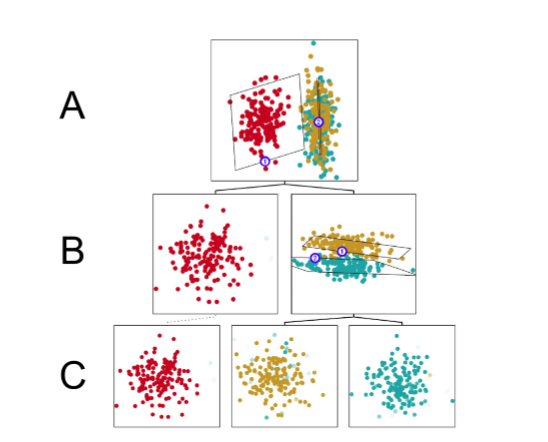
\includegraphics{figs/hierarchy_bishoptipping.png}
    \caption[Example of a hierarchical cluster structure.]{\small \textbf{Example of a hierarchical cluster structure.} \small The top-level shows the complete data-set in its latent space (A). The data is then clustered into a red and a yellow-and-blue cluster, and the latent space of each of those clusters is given (B). Doing so reveals structure within the yellow-and-blue cluster that was not visible before. This allows the cluster to be divided even further into separate yellow and blue sub-clusters (C). This figure has been copied from Bishop \& Tipping (1998) \cite{bishop1998hierarchical}.}
    \label{fig:example_hierarchy}
\end{figure}

In this case, $\mathcal{G}_i$ is the set of second-level sub-clusters $j$ that are contained within top-level cluster $i$. The complete-data log-likelihood function of this model is similar to that of a MoPPCAs model. %Note that the term $\pi_j$ is omitted. This is because the second layer of the hierarchical mixture model is initialized after the top-level MoPPCAs. Therefore, $\pi_j$ has already been estimated and so it remains constant over the whole function.

\begin{equation}\label{eq:llh_hmppca}
    \sum^n_{i=1} \sum^K_{j=1} \gamma^j_i \sum_{m=1}^{|\mathcal{G}_i|} \gamma_i^{m|j} \ln{\pi_{m|j} p(\bm{x}_i, \bm{z}_i)}%\mathcal{N}(\bm{x}_i|\bm{W}_m\bm{z} + \mu_m, \sigma^2_m\bm{I})}
\end{equation}

\section{Stan, NUTS and ADVI}\label{sec:stan}

All models described in this report have not been fitted analytically or by use of the EM algorithm as described above. Instead, all statistical models have been programmed in Stan so that they could be solved numerically. Stan is a platform for statistical modelling. An example of a PPCA model as defined in Stan is given in Appendix \ref{AP:ppca_stan}. Given a statistical model, Stan tries to find the posterior distribution of all unknown `parameters'. These parameters might be parameters in the classical sense, e.g. the mean and standard deviation of a Gaussian given the observed data. Alternatively, they might be missing variables, e.g. the latent variables explaining the observed variables. Using Stan has several advantages. It allows us to specify a model, or just its log-likelihood function, and then Stan attempts to find the optimal solution without requiring to derive the equations to find the maximum-likelihood solution to the model. This is especially useful when manipulating a statistical model, as we can adjust the model without needing to rewrite the (algorithmic) solution. Secondly, Stan makes use of samplers which not only give a point estimate for the parameter values but the entire posterior distribution of each unknown parameter. This gives us information about the uncertainty of the found solution. Stan implements two main algorithms for this. Most notably, Stan makes use of the No U-turn sampler (NUTS) (discussed in Section \ref{sec:nuts}). This is an extension of Hamiltonian Monte Carlo sampling. NUTS has the benefit over Hamiltonian Monte Carlo that it automatically determines the number of steps needed for convergence, saving computation time. The other, more recently implemented algorithm to determine the posterior of the parameters, is the automatic differentiation variational inference (ADVI) algorithm (see Section \ref{sec:advi}). This is an algorithm based upon variational inference. It selects a distribution from a variational family that is as similar as possible to the posterior. This might be less exact, but it saves a lot of computational cost without affecting the accuracy of the outcome too much. These algorithms were both utilized and compared in this project.

Stan does not stand alone, but rather, it needs to be implemented in another environment. For this project, programming was done by use of Python, in which Stan was implemented through a package called PyStan \cite{stan2018pystan}. The general workflow is as follows. Data is read in through the Python environment and a statistical model is specified in Stan. Then the model is compiled. Using the data as input, Stan is used to infer the parameters and outputs them to the Python environment. This data is then finally analyzed using Python.

\subsection{Monte Carlo sampling and NUTS}\label{sec:nuts}
Monte Carlo (\textbf{MC}) methods are a branch of sampling methods. They are forms of Markov chains, and generally entail a random trajectory through the sample space, directed by the underlying probability distribution of interest. An easy and well-known example is the Metropolis-Hastings algorithm \cite{metropolis1953equation, hastings1970monte}, where a fictive particle jumps randomly to new positions within the sample space. Based on the ratio of the probabilities of the old and new position, a new position can be accepted as a sample. If it is rejected, a jump to a new position is made. The samples drawn using this algorithm are guaranteed to converge to the underlying distribution when sampling long enough.

A drawback of this algorithm is that the number of samples necessary for convergence is sub-optimal, as the random walks through the sample space are inefficient. For this reason, other algorithms, such as Hamiltonian Monte Carlo (\textbf{HMC}), were proposed \cite{duane1987hybrid}. When using HMC, the fictive particle behaves as in a Hamiltonian dynamics simulation. A particle has a position in the sample space and a velocity. For a pre-determined number of steps of fixed step size, the particle moves in a random manner through the sample space, at the end of which the position is either accepted or rejected as a sample. This algorithm produces much more efficient random walks and is therefore less costly computationally. However, this algorithm has its own drawbacks. HMC requires manually setting a step-size parameter $\epsilon$ and a number of steps $L$. Sub-optimal values for these parameters can result in unnecessary computational cost and inaccurate results. Particularly, setting $L$ too high will result in the particle slowly returning to its original position, which requires not only unnecessary computation but also leads to slower convergence. Tuning these parameters usually requires some degree of expertise and a few tuning runs of the algorithm. Some adaptations to HMC have been proposed to automatically tune $\epsilon$ \cite{nesterov2009primal}, but not $L$.

The No-U-Turn Sampler \cite{hoffman2014no} (\textbf{NUTS}) is an extension to HMC. NUTS is most notable for its ability to determine the optimal number of steps $L$ while running. When a particle moves through the sample space to generate a sample, the number of steps needs to be high enough for a decent random walk to happen, but not too high as the fictive particle will eventually loop back and move back to its original position. The point where the fictive particle is the furthest away from its initial position is characterized by sharp turns in the path of the particle. Stopping at these `U-turns' is where the algorithm has drawn its name from. Additionally, NUTS tunes $\epsilon$ automatically whilst running the algorithm.

% To optimize the number of steps, the optimal number of necessary steps for the algorithm to run is determined while running. Each sample is initialized with the position of the previous sample and then walks a trajectory to the next sample. 
% In the optimal case, the next sample is chosen when the new sample is as far away as possible from the old sample. If the number of steps of the trajectory is set too low, the fictive particle has yet to reach this farthest point, whereas if the number of steps is too large, the particle returns in the direction of its original position, wasting both computation and decreasing the efficiency of the algorithm. 
NUTS has added a feature that checks when the sampling trajectory is at its maximum length and then uses this criterion to stop. The concrete criterion depends on the derivative of half the squared distance from the original to the new sample. If this measure is close to zero, the squared (and thus the absolute) distance between the two samples is not changing anymore and the trajectory is probably at its point of return. The series of samples is desired to be a Markov chain. One necessary property of such Markov chains is known as time-reversibility, i.e. the validity of the series of samples is not dependent on whether the samples are read from front to back or back to front. To maintain the time-reversibility of the Markov Chain, the trajectory is run both forward and backward in time. The algorithm builds a `tree' to examine the structure of the trajectory and the algorithm halts with a probability that is negatively proportional to the derivative of half the squared distance at either end of the trajectory. 
Secondly, NUTS tunes $\epsilon$ on-the-fly, based on a method named `dual averaging' \cite{nesterov2009primal}. This adaptation has been slightly improved to include more parameters. Apart from adapting $\epsilon$ while running, NUTS does a quick search for a reasonable value of $\epsilon$ to initialize the algorithm with.

 \subsection{Variational inference and ADVI}\label{sec:advi}
 Variational inference (\textbf{VI}) is a method of approximating a posterior probability distribution $p(\bm{\theta}|\bm{x})$ for the parameters $\bm{\theta}$ given data $\bm{x}$ that is difficult to determine. It works by chossing a familiy of probability distributions $q(\bm{\zeta})$ and then minimizing the dissimilarity between $P$ and $Q$. To measure this dissimilarity, the Kullback-Leibler divergence of $P$ and $Q$ ($D_{KL}(Q||P)$) is used. This is an asymmetric similarity measure defined as $D_{KL}(Q||P) = \int q(\bm{\theta}) \log{\frac{q(\bm{\theta})}{p(\bm{\theta}|\bm{x})}}$. This can be rewritten as $D_{KL}(Q||P) = \log{p(\bm{x})} - \mathcal{L}(Q)$, where $\mathcal{L}(Q) = -E_{\bm{\theta}}[\log{q(\bm{\theta})}-\log{p(\bm{\theta},\bm{x})}]$. The first term $\log{p(\bm{x})}$ is known as the evidence. The last term $\mathcal{L}(Q)$ is the evidence lower bound or \textbf{ELBO}. Its name is derived from the fact that the evidence is the sum of the ELBO and the KL divergence; since the KL divergence is non-negative, the ELBO is the lower bound for the evidence.
 Often, finding the optimal distribution $q(\bm{\zeta})$ though KL-divergence minimization is difficult or impossible. However, the evidence is a function that does not rely on $q(\bm{x})$ and is therefore kept constant as $q(\bm{x})$ is optimized. Minimizing the KL divergence is therefore equivalent to maximizing the ELBO, as is done in VI.
 
 ADVI \cite{kucukelbir2017automatic} is an algorithm that implements VI and automates the process. Traditionally, performing a VI algorithm required that the researcher had specified a VI algorithm beforehand, which included the selection of a family of variational distributions, the objective function to optimize and the computation of its gradients. This was not only an effort to the researcher, but it was also an obstacle to the automatization of the process. ADVI differs in that it transforms the given model to be suitable to a premade VI algorithm so that the aforementioned steps become obsolete.
 ADVI starts off by transforming the probability density function of the posterior. ADVI's VI algorithm assumes that all parameters live in the real space and are unconstrained, which is what is achieved by this transformation. After this transformation, ADVI's premade VI algorithm can be used for ELBO maximization.
 
 A family of variational approximations is expressed as Gaussians, either with a diagonal covariance matrix (mean field variational inference) or with a full covariance matrix (full-rank variational inference). The latter is more precise but also computationally more costly. 
The objective function to be optimized is expressed as the expectation of the distribution, which can easily be derived by sampling from the distribution and taking the empirical mean.
%  Seeing as how a variational distrbution consists out of Gaussians, computing the expectation of each distribution can be done through Monte Carlo (\textbf{MC}) integration and requires only sampling from the distribution and taking the mean of the sample.
%  Seeing as how easy it is to compute the expectation of a variational approximation, the gradient of the objective function is expressed as an expectation over $q$. This allows MC methods to easily approximate the gradient. By use of elliptical standardization, this expectation is expressed by standard Gaussians, which are easy to evaluate.
 
 The gradient of the logarithm of the joint probability distribution of the parameters and the data with respect to the parameters ($\nabla_\theta \log{q(\bm{x},\bm{\theta})}$) is computed through automatic differentiation \cite{baydin2017automatic}. Automatic differentiation is a technique to determine the gradient of a function which has been implemented in Stan (and was one of the reasons that Stan was chosen as a suitable environment for ADVI).
 Using the expectation of the gradient of the log joint probability, it is possible to obtain a noisy estimate of the gradients of the ELBO.
 The noisy gradient of the function is then used to optimize the variational distribution $q$ by stochastic gradient ascent. Finally, the ELBO has been maximized and a (local) optimum for the posterior distribution of the parameters has been found. This sequence of steps is integrated in PyStan under the name Variational Bayes (\textbf{VB}) and will be referred to under this name in this report.
 
 
 \section{Detailed description of the model}\label{sec:mode}
\subsection{The model}
Our visualization model is a hierarchical one, based on an earlier model by Bishop \& Tipping \cite{bishop1998hierarchical} (see Figure \ref{fig:example_hierarchy}). It visualizes data, and if group structures are present, it attempts to find groups within the data on the top-level, and then possibly sub-groups within the groups at the deeper levels. The model presented in this report is mainly used for visualization of data. Therefore, the model was built to find the latent space of the data on every level, so that the data could be represented in its latent dimensions. The first latent data-space, on top-level, can easily be obtained with a normal PPCA model. The result gives the projection of the data on the first two principal components. Next, a MoPPCAs model is applied to the data, which attempts to find clusters and gives their projection onto their first two principal components. From this point on, the model repeatedly applies MoPPCAs to every cluster of data for the desired number of levels. For every level, the algorithm evaluates the clusters found on the level above. First, every cluster is tested for how many sub-clusters it possibly contains. If the cluster contains two or more sub-clusters, a MoPPCAs is initialized. If the cluster contains only one sub-cluster, i.e. the cluster cannot be divided any further into sub-clusters, its branch is marked as fully analyzed. Once the MoPPCAs returns the results, we have the new latent spaces of the cluster of interest. The MoPPCAs gives us also the probabilities of all the data-points belonging to the sub-cluster $\gamma^k_i$ (see equation \ref{eq:gamma}). When all clusters have been divided into their sub-clusters, the next level is initiated, where every cluster of the last level will be attempted to split into its sub-clusters. The researcher has the possibility to select using NUTS or VB for fitting the PPCA and MoPPCAs models before initializing the model.

Note that, even though every MoPPCAs model returns the latent spaces of the found sub-clusters, the full-dimensional data is used as input to these models. The found latent data is not reused as input for later MoPPCAs models. The latent space is only used for visualization purposes (Section \ref{sec:visualization}) and for estimation of the number of sub-clusters (Section \ref{sec:n_clus}).

Clusters that are found to be fully analyzed do not undergo further evaluation on deeper levels. Instead, the latent data-set is copied over to the next level directly. When all clusters are fully analyzed or when the maximum depth of levels as specified by the researcher is reached, the model stops. A summary in pseudocode for this model is given in Algorithm \ref{alg:model}.


\begin{algorithm}[H]
 \KwData{$X$}
 \KwResult{$\bm{Z}$ and $\gamma^j_i$ for all data-points $\bm{x}_i$ and clusters $j$}
%  initialization\;
initialize $level := 0, max\_depth = 5, max\_tries = 3$\;
 Initialize top-level PPCA and plot latent projection\;
 Make every data-point part of one cluster $c$ with $\gamma^c_i=1.0$\;
 \While{$level < max\_depth$}{
 Increment $level := level + 1$\;
 \For{every cluster $c$ found in last level}{
 Find initial clustering with GMM in latent space\;
 \If{there are no sub-clusters}{
 skip to next cluster}
 \While{No MoPPCAs solution has been found}{
 Set $tries := 0$\;
 \While{$tries < max\_tries$}{
 Increment $tries := tries + 1$\;
 Initialize weighted MoPPCAs model on full-dimensional data-set with weights $\gamma^c_i$\;
 \If{MoPPCAs find model with same number of clusters as initial GMM}{
 Break loop}
 }
 \If{No MoPPCAs fit is found with same number of clusters as GMM}{
 Break loop and use MoPPCAs fit with highest number of clusters as initialization for new MoPPCAs model}
 }
 \For{every sub-cluster $sc$ found with MoPPCAs model}{
 Extract probabilties $\gamma^{sc}_i$\;
 $\gamma^{sc}_i := \gamma^{sc}_i \gamma^{c}_i$\;
 Plot found latent data-set with ink density proportional to $\gamma^{sc}_i$\;
 }
 }
 }
 \caption{Pseudocode of HmPPCAs model}
 \label{alg:model}
\end{algorithm}



\subsection{Drawing a sample}
 When NUTS is used, the user receives the samples that were generated in the process. This excludes the first warm-up samples and every other sample is thrown away as well to reduce the correlation between samples, but the other samples are returned to the user. With the settings used in this project, this left $300$ samples for the user. When VB has found its optimal posterior distribution, a sample of $1000$ points is taken from the distribution. In either case, the mean of all generated data-points is taken as the expected value of the unknown parameters. When the latent data-set or other parameters are computed, then these expected values were used.

\subsection{Initialization, priors and constraints for the MoPPCAS models}\label{sec:prios}
The MoPPCAs model was highly dependent on the initialization. This is mainly due to local optima in (soft) clustering methods. The first trials of the MoPPCAs models were performed with Stans default random initialization of parameters. This would often lead to high computation times and implausible solutions. A common result was that the algorithm would find values of $\pi_k$ that were near zero for one or more clusters. This meant that no data-points or only a few outliers were determined to be part of that cluster, which made them practically absent. Part of the reason that this happened is that a normal distribution with a very low spread can be fit to a cluster containing only one data-point with a very high likelihood. The spread of the remaining cluster(s) would be set high enough to encompass the remaining data-points. To prevent this behaviour, the initial clustering was performed by a GMM. GMMs were fitted in the latent space while varying the number of components. The optimal number of components was determined using the Bayesian information criterion (\textbf{BIC}; see Section \ref{sec:n_clus}) and was used as a reference for the MoPPCAs clusters. After the GMM clustering completed, only the most probable cluster for each data-point was noted, not the probabilities of belonging to each cluster. The values of $\mu_k$ and $\sigma_k$ were inspired by the values of the centers and the spread of the clusters as found by the GMM. Because the GMM clustering was performed in the latent space, the labeling of the data-points to their clusters had to be applied to the same data-points in the full-dimensional space first. This way, the center and covariance matrix of each cluster could be estimated in the full-dimensional space. Basing $\sigma^2$ on the covariance matrix of the clusters is not entirely correct, because the covariance matrix of the PPCA model is $\bm{W}\bm{W}^T + \sigma^2 \bm{I}$. Directing the value of $\sigma^2$ to values based on the found covariance matrix would actually overestimate $\sigma^2$, which in turn would lead to underestimation of $\bm{W}$. However, the resulting inference of the model would be off without doing so. Therefore, after trying various alternatives, the following three steps were taken to direct $\sigma^2$ to the spread of the clusters as found by the GMM.

First of all, the centers and the spread of the clusters that were found by the GMM were used to initialize parameters $\mu_k$ and $\sigma_k$ in the MoPPCAs model. Values for $\pi_k$ were computed from the GMM solution and used as initial values for $\pi_k$ similarly. The solution of the GMM was also used to initialize $\gamma^k_i$ for all values as  $1$ (when $i$ belonged to $k$ according to the GMM) or $0$ (otherwise). It was then evaluated whether the problem where few to no data-points were assigned to a cluster was avoided. The problem was solved for low-dimensional data-sets, but the problem persisted when more complex data-sets were analyzed. Another reason for this initialization was that a random initialization would lead to random labeling of clusters. This would lead to inconsistencies in cluster labels between samples and affect the outcome negatively. A consistent initialization meant also that the label-swapping problem during clustering was solved.

Secondly, a prior was set over $\mu_k$ and $\sigma_k$, to direct the parameters towards the correct solution. For $\mu_k$, a prior was specified in the form of a normal distribution that was fit to the points that the GMM had labeled to cluster $k$ in the full-dimensional space. As a prior for the standard deviation of the clusters, an inverse gamma distribution, fit with help of the GMM solution, was specified at first, but this seemed to worsen the results. A normal distribution was then specified as a prior as this yielded better results. Since $\sigma_k$ is a single value related to the spread in all dimensions within that cluster, the mean of the diagonal of the covariance matrix of a cluster was used as the expectation of $\sigma_k$, thus $E[\sigma_k] = \frac{1}{d}Tr(\Sigma^{GMM}_k)$ with $\Sigma^{GMM}_k$ being the covariance matrix of GMM cluster $k$.
% The standard deviation of the prior distribution was set to be the standard deviation of all diagonal entries in $\Sigma^{GMM}_k$.
This approach saved computational cost, but it did not necessarily prevent the problem discussed above.

Since the problem of empty clusters resulted in clusters with a minimal or large spread, constraints were set on the standard deviations of the MoPPCAs clusters in the data space. Therefore, a lower bound on $\sigma_k$ was set of $0.75$ times the standard deviation of the GMM cluster in the dimension with the lowest spread. This did not prevent the problem, as there could still be clusters with near-zero $\pi_k$, while other clusters took over their data-points by increasing their $\sigma_k$. Therefore, an upper bound was also set on the value of $\sigma_k$. This upper bound was set to be $1.25$ times the standard deviation of the GMM cluster in the dimension with the largest spread. Stan does not accept different constraints on the entries of one vector and our lower and upper bounds were different for every cluster. As a solution, \textit{raw} vectors of $\bm{\mu}_k$ and $\sigma_k$ were evaluated as normalized vectors with entries between $0$ and $1$. Now, they all had the same upper and lower bounds ($1$ and $0$). These normalized values were then later in the model transformed to their real values by multiplying them with the difference between the upper and lower bound values and adding the lower bound values to them.

Using all these constraints put the initial GMM solution largely in charge of the clustering part of the MoPPCAs solution, leaving the MoPPCAs model to make only minor adjustments to the clustering of the full-dimensional space. Despite this, it still happened occasionally that `empty' clusters were found and that the MoPPCAs model found a different optimal clustering with fewer clusters. This was not necessarily a problem on the side of the MoPPCAs model, because overestimation of the number of clusters also happened from time to time (see Section \ref{sec:n_clus}). If this happened three times in a row, the MoPPCAs solution with the highest found number of clusters was accepted. However, because this model was initialized with a prior directed at a different solution, a second MoPPCAs model was initialized with the newly found number of clusters. All initial values were copied from the first MoPPCAs model, and priors and constraints on the model were taken from the first MoPPCAs solution in the same way that they were taken from the initial GMM for the first MoPPCAs model.

\subsection{Dealing with responsibility terms on the deeper levels}
When analyzing a cluster, every data-point $i$ has a responsibility term $\gamma^k_i$, describing the probability of belonging to cluster $k$. Therefore, all data-points are input to the MoPPCAs, even the ones that probably don't belong in this cluster, albeit with a very low weight. These numbers are passed into the MoPPCAs to be used in the expected complete-data log-likelihood of equation \ref{eq:llh_hmppca}. For the first level, $\gamma^k_i = 1$ for all data-points, meaning that every data-point starts as being part of the same cluster with complete certainty. When we move to deeper levels, the likelihood equation changes from \ref{eq:llh_hmppca} to \ref{eq:llh_hmppca2}, where $l$ sums over the sub-clusters at the next level.

\begin{equation}\label{eq:llh_hmppca2}
    \sum^n_{i=1} \sum^{K_1}_{j=1} \gamma^j_i \sum^{|\mathcal{G}_j|}_{l=1} \gamma^{l|j}_i \sum_{m=1}^{|\mathcal{G}_l|} \gamma^{m|j,l}_i \ln{\pi_{m|j,l} p(\bm{x}_i,\bm{z}_i)}
\end{equation}

Noting that $\gamma^j_i \gamma^{l|j}_i = \gamma^{j,l}_i$ we can rewrite \ref{eq:llh_hmppca2} back to \ref{eq:llh_hmppca}, where now $j$ denotes the sub-clusters on the next level. We can, therefore, reuse the same MoPPCAs model, but this time inputting the probabilities of belonging to the new sub-clusters as $\gamma^j_i$. Every MoPPCAs returns $\gamma^{l|j}_i$. Seeing as how $\gamma^j_i \gamma^{l|j}_i = \gamma^{j,l}_i$, we just have to multiply this number with the probability of belonging to the cluster on the level above to obtain the probability of belonging to the new sub-cluster, which will be the input responsibility term for the next level. Therefore, the model initializes a vector of ones of length $n$ as the responsibility terms, inputs it to the MoPPCAs model and then multiplies it element-wisely with the output responsibility terms to obtain the new responsibility terms used for the MoPPCAs for the new sub-clusters on the next level.


\subsection{BIC score to assess the number of clusters}\label{sec:n_clus}
The number of clusters to be found was estimated using the Bayesian information criterion (\textbf{BIC}). The data was clustered by a GMM with various values for the number of clusters. For the GMM models, a ready-to-use GMM package 'GaussianMixture' from the `Sklearn' package was used, as it worked faster than Stan and we needed only a simple estimate for initialization, not the whole posterior of all parameters. Data-points were assigned to the plot with their highest responsibility term and only the points assigned to a plot were included in the GMM. These GMMs were estimated on the latent data. Although the full-dimensional data may contain more information, it also contains more noise and we found that better estimates were therefore obtained from using the latent data. The maximum number of clusters to be found, $K_{max}$, was set relatively low to $K_{max} = 3$. This lead to the need for multiple levels in our models, to get a better grasp of the hierarchical working of the model. The minimum number of clusters to be found $K_{min}$ was always set to $1$, except for the top-level, where it was set to $2$ to stimulate the model to make at least one division in the data-set. For each value of $K$, three GMM models were fit to the data, although users can choose to fit as many GMM models as they like. Pseudocode for this process is given in algorithm \ref{alg:n_clus}. Note that $Z$ in this algorithm contains not all data-points in the latent space, but only the ones that were assigned to the plot which is analysed. 

The BIC of a model fit is defined as $BIC = k \ln{n} - 2 \ln{\mathcal{L}}$, where $n$ is the number of data-points, $k$ the number of clusters and $\mathcal{L}$ the likelihood. The likelihood of a GMM model is defined in Appendix \ref{app:gmm_em}. For each model, the BIC was computed, and the model with the lowest BIC was chosen as the best suitable model for the data.
% Not only was the number of optimal sub-clusters directed to the following MoPPCAs model, the model was also initialized with all data-points labeled accordingly to the best found GMM model. The mean and standard deviations of all clusters were also given to the model, after being recomputed in the original, full space. 

Even though the BIC score usually gave a very good estimate for the number of sub-clusters, it happened from time to time that the MoPPCAs found fewer clusters. In these cases, the responsibilities were all approaching $0$ for every data-point for that cluster. If a sub-cluster $j$ was not assigned any data-point $i$ (i.e. $\text{argmin}_k \gamma^k_i) \neq j~\forall i$), the MoPPCAs was retried for up to three times. If the suggested number of sub-clusters was still not found by the third time, a new MoPPCAs model was initialized that looked for fewer sub-clusters. After all, it is possible for the GMM to over-estimate the number of sub-clusters. Under-estimation of the number of sub-clusters is not a problem since the found sub-clusters will be analyzed further at deeper levels.

\begin{algorithm}[H]
 \KwData{$Z$, $K\_min$, $K\_max$, $n\_ref$}
 \KwResult{GMM fit on $Z$ with optimal number of clusters}
Initialize $k = K\_min$\;
 \While{$k \leq K\_max$}{
 set $ref := 0$\;
 \While{$ref < n\_ref$}{
 increment $ref := ref + 1$\;
 Cluster $Z$ into $k$ clusters using GMM\;
 Compute likelihood $L$ of the resulting GMM fit\;
 Compute the BIC as $BIC := k \ln{n} - 2 \ln{L}$\;
 }
 }
 Return GMM fit with lowest BIC\;
 \caption{Determining the number of clusters}
 \label{alg:n_clus}
\end{algorithm}
